\documentclass[conference]{IEEEtran}
\usepackage{cite}
\usepackage{graphicx}
\usepackage{amsmath,amssymb,amsfonts}
\usepackage{textcomp}
\usepackage{url}
\usepackage[hidelinks]{hyperref}
\usepackage{xcolor}
\emergencystretch=3em
\setcounter{dbltopnumber}{2}
\renewcommand{\dbltopfraction}{0.95}
\renewcommand{\dblfloatpagefraction}{0.85}
\renewcommand{\textfraction}{0.05}
\newcommand{\CADDAM}{CADD\allowbreak{}+\allowbreak{}AlphaMissense}
\newcommand{\GCNCADDAM}{GCN\allowbreak{}+\allowbreak{}CADD\allowbreak{}+\allowbreak{}AlphaMissense}

\title{Auditing PPI Graph Augmentation for Missense Variant Pathogenicity Prediction under Topology, Connectivity and Homology Constraints}

\author{\IEEEauthorblockN{Yuxin Tian, Xianguo Zhang\textsuperscript{*}, Weibo Meng, Jieqi Yin, and Yongqin Jin}
\IEEEauthorblockA{College of Computer Science (College of Software), College of Artificial Intelligence\\
Inner Mongolia University, Hohhot 010021, China\\
Email: yuxin\_t02@163.com; 2595083628@qq.com\\
\textsuperscript{*}Corresponding author: Xianguo Zhang}}
\hypersetup{pdfauthor={Yuxin Tian, Xianguo Zhang, Weibo Meng, Jieqi Yin, Yongqin Jin}}



\begin{document}
\maketitle


\begin{abstract}
\bfseries\boldmath
Protein interaction networks may add context to missense variant prediction, but gains depend on the evaluation design. We audit fixed two-hop protein-feature propagation (FPP), without learned graph parameters, using 177,213 ClinVar variants on one STRING functional-association network. Matched three-seed comparisons gave mean AUC 0.7835 for raw ESM and 0.7950 for full FPP. We matched propagation operators, classifier seeds, training budgets and validation-based selection across direct-edge and topology-permutation controls. Protein-clustered intervals for the primary gain crossed zero. With CADD and AlphaMissense, real-network fusion exceeded raw-feature fusion, while its margin over edge-ablated fusion remained uncertain. Intervals condition on fitted ensembles. Under homology-aware splitting, three matched seeds per fusion arm gave AUC 0.9755 for the score baseline and 0.9752 with FPP. Topology subgroups and prediction transitions remain exploratory. The audit supports explicit controls and split-aware uncertainty; it does not establish limits on trained graph models or generalize beyond this dataset and network.

\end{abstract}

\begin{IEEEkeywords}
\bfseries\boldmath
Missense variant pathogenicity, STRING networks, fixed feature propagation, protein language models, evaluation audit.
\end{IEEEkeywords}

\section{Introduction}

Missense variant pathogenicity prediction has been advanced by established methods such as CADD, REVEL, MVP, PrimateAI, EVE and AlphaMissense \cite{Kircher2014CADD,Ioannidis2016REVEL,Qi2021MVP,Sundaram2018PrimateAI,Frazer2021EVE,Cheng2023AlphaMissense}, as well as by protein language models such as ESM \cite{Lin2023ESM}. These approaches capture sequence, evolutionary and annotation-derived signals. Disease-associated proteins are also embedded in molecular interaction networks, and disease-associated mutations can perturb protein-protein and other macromolecular interactions \cite{Barabasi2011NetworkMedicine,Menche2015DiseaseModules,Sahni2015InteractionPerturbation,Chen2018InteractomePerturbation}. PPI graphs provide an additional source of context for missense variant prediction.

Earlier approaches incorporated protein-interaction and other molecular-network features into single-amino-acid variant prioritization, showing that network context can provide information complementary to sequence, structure and annotation features \cite{Yates2014SuSPect,Ozturk2022NetworkFeatures}. More recent graph-based variant predictors include graph attention models for missense effects, heterogeneous gene-variant graph approaches, multimodal variant graph methods and disease-specific graph models \cite{Zhang2022gMVP,Cheng2021VEGN,Yu2025GNNMAP,Ghadie2025DiseaseSpecificGNN}. These studies establish the relevance of relational structure to variant interpretation. We focus on how to interpret gains obtained by propagating protein language model embeddings over a shared STRING association graph before variant-level classification.

A shared-graph setting mixes several effects. Train, validation and test variants may have distinct protein identifiers while their proteins remain directly connected in the same STRING graph. Related proteins may also cross partitions when homology is not explicitly controlled \cite{Littmann2022ProteinMLTips,Teufel2023GraphPart}. Strong variant-effect predictors such as CADD and AlphaMissense can further reduce the marginal contribution of graph propagation. We evaluate protein-topology correspondence, graph connectivity, protein-level uncertainty, homology-aware performance and complementarity to established predictors.

We audit raw ESM, fixed propagation, external scores and fusion models on a reconstructed ClinVar-STRING dataset. The contribution is an evaluation study: it combines graph-intervention controls with capacity-matched fusion and protein-clustered uncertainty, documents sensitivities to split and comparison protocol, and describes exploratory topology and error-transition profiles. The audit does not introduce a new predictor or cover trained message-passing architectures.

\section{Materials and Methods}

\subsection{Dataset and graph construction}

ClinVar variant annotations were obtained from the official NCBI ClinVar FTP tab-delimited variant-summary file \cite{Landrum2020ClinVar}. We used the ClinVar variant-summary release dated 31 March 2024 and retained checksums for the exact input file used in the reconstruction. We reconstructed a filtered, non-conflicting missense dataset and mapped variants to STRING human protein identifiers. We retained GRCh38 germline missense SNVs with criteria-supported review status, combined pathogenic and likely pathogenic records into the positive class, combined benign and likely benign records into the negative class, removed uncertain or conflicting records, and collapsed duplicate VariationIDs. The final ClinVar-STRING dataset contained 177,213 missense variants mapped to 14,123 labelled STRING proteins. The propagation graph contained 19,622 STRING protein nodes and 13,715,404 directed edge-index entries from the STRING v12 protein-association network \cite{Szklarczyk2023STRING}. We used this network as STRING network context; its association evidence extends beyond direct physical interactions.

\subsection{Protein representations and fixed propagation}

Raw protein features were generated using the ESM-2 650M checkpoint, with 1,280-dimensional protein-level vectors obtained by residue averaging \cite{Lin2023ESM}. Fixed protein-feature propagation (FPP) was computed by two-hop GCN-style propagation over the normalized STRING graph \cite{Kipf2017GCN}. FPP has no learned graph-convolution parameters; the downstream MLP alone was trained. Fixed propagation isolates topology-induced smoothing from capacity gains due to trainable graph layers and provides a controlled representation for the audit. Let $X$ denote the raw ESM protein-representation matrix. The matched implementation adds self-loops before symmetrizing the retained edge list and sums duplicate contributions when coalescing. Thus $\tilde{A}=(E+I)+(E+I)^{\mathrm{T}}$, where $E$ is the edge-index count matrix; STRING combined scores are not propagation weights. Let $\tilde{D}$ denote its weighted degree matrix. We computed the symmetrically normalized adjacency matrix as
\begin{equation}
\hat{A}=\tilde{D}^{-\frac{1}{2}}\tilde{A}\tilde{D}^{-\frac{1}{2}},
\end{equation}
\begin{equation}
H=\frac{1}{3}\left(X+\hat{A}X+\hat{A}^{2}X\right).
\end{equation}
The fixed two-hop FPP representation $H$ averages the original ESM features, one-hop and two-hop STRING-smoothed features. Propagation used only graph structure and ESM features; downstream classification used the representation of each variant's mapped STRING protein. The full graph contained train, validation and test nodes with their ESM features, making the evaluation transductive. Held-out features and graph structure were available during propagation, but held-out labels were not used. Embedding-only models assign identical inputs to variants mapped to the same protein; they cannot resolve residue-specific effects within that protein.

\subsection{Splits, classifiers and external predictors}

The original split assigned train, validation and test variants by STRING protein ID, with no shared proteins across partitions. The split contained 141,864 training variants, 17,129 validation variants and 18,220 test variants. The homology-aware split used MMseqs-derived protein clusters, assigned each cluster wholly to one partition by greedy balancing of variant-row counts, without label-prevalence stratification, and preserved the same row counts \cite{Steinegger2017MMseqs2}. We use this split as a stress test. Its test positive rate was 10.56\%, compared with 31.95\% in the original split, which limits direct cross-split AUPRC comparison.

All representation and fusion models were evaluated with a downstream MLP classifier selected by validation AUC and optimized with Adam \cite{Kingma2015Adam}. Multi-feature representation and fusion models used a 512/128 hidden-layer MLP with dropout 0.3. Historical low-dimensional external-score baselines used a smaller 32/16 classifier with dropout 0.2. Architecture-matched \CADDAM{} and fusion-control comparisons used the 512/128 classifier to keep downstream capacity matched. Training used mini-batches of 1,024 variants, learning rate $10^{-3}$, weight decay $10^{-5}$, a maximum of 50 epochs in every new matched arm and early stopping after five consecutive validation checks without improvement in validation AUC. Class imbalance was handled with \texttt{BCEWithLogitsLoss} using training-partition positive-class weight $N_{\mathrm{negative}}/N_{\mathrm{positive}}$. CADD GRCh38 v1.7 scores and AlphaMissense hg38 scores were matched to the reconstructed variants \cite{Kircher2014CADD,Schubach2024CADDv17,Cheng2023AlphaMissense}. CADD scores covered 177,205 variants (99.995\%), and AlphaMissense scores covered 171,753 variants (96.92\%). Missing CADD and AlphaMissense scores were imputed with training-set medians; AlphaMissense-based feature sets also included a binary missingness indicator. In the evaluated MLP configurations, no additional z-score standardization was applied to CADD, AlphaMissense or embedding-derived inputs. All architecture-matched fusion controls shared the same preprocessing and feature construction. Alternative feature-scaling strategies were not evaluated. All new matched arms used classifier seeds 42, 43 and 44, the same 50-epoch limit and validation rule. Permutation arms combined graph seeds 6042--6044 with each classifier seed. Historical results retain their original protocols (Supplementary Tables 8 and 11).

\subsection{Audit analyses}

Uncertainty was assessed using variant-level bootstrap and protein-clustered bootstrap \cite{Efron1993Bootstrap}. Connectivity tests removed direct train-test STRING edges and regenerated FPP embeddings. Partial edge-ablation curves removed 0\%, 25\%, 50\%, 75\% and 100\% of direct train-test protein pairs using random removal, higher-STRING-score-first removal and lower-STRING-score-first removal. Topology permutation preserved the unlabeled graph structure and randomized the correspondence between protein identity and graph position, testing whether generic graph smoothing explained the gain. Fusion controls concatenated \CADDAM{} features with raw ESM, edge-ablated FPP and topology-permuted FPP representations, testing representation complementarity and sensitivity to protein-topology correspondence. Edge removal also changes normalization and retains indirect cross-partition paths; it does not isolate a causal contribution of direct connectivity.

An implementation audit found that historical full FPP added loops before symmetrization, whereas old graph controls added a single loop after adding reverse edges. New representation and fusion controls were regenerated using the common full-FPP operator, with frozen protein features and partitions retained. This corrects an additional comparison mismatch; the old partial-ablation curve remains historical and descriptive. The restored runtime used Python 3.10.8, PyTorch 2.1.2 with CUDA 11.8, NumPy 1.26.4 and one RTX 4090. Input hashes, split alignment and a numerical propagation check preceded training.

Topology-context analyses stratified test variants by degree, k-core, betweenness, clustering coefficient, neighbour-risk and community-boundary features. Neighbour-risk and neighbour pathogenic-rate features for validation and test proteins were computed from training-set labels only; validation and test labels were not used to construct these topology-context features. Corrected-sample analyses compared variants whose predictions were corrected or degraded after adding graph context. Multiple topology-feature comparisons used Benjamini-Hochberg false-discovery-rate correction \cite{Benjamini1995FDR}. All topology strata are post-hoc test-set descriptions. Selected joint-cell intervals do not adjust for subgroup selection. The so-called difficulty-matched analysis in the original draft actually stratified by baseline error type; it did not match continuous prediction scores. AUPRC was interpreted within each split because precision-recall metrics are sensitive to class prevalence \cite{Saito2015PrecisionRecall}.

\begin{table}[t]
\caption{Run provenance for the main results. Historical and matched protocols are in Supplementary Tables 8 and 11. Runs count fitted classifiers, not bootstrap resamples.}
\label{tab:run_sources}
\centering
\footnotesize
\setlength{\tabcolsep}{3pt}
\renewcommand{\arraystretch}{1.12}
\begin{tabular}{p{0.40\columnwidth}p{0.14\columnwidth}p{0.36\columnwidth}}
\hline
Evidence & Runs & Summary used \\
\hline
Fig. 1B,D/F representations & 3/arm & Matched seeds/operator/budget \\
Fig. 1C uncertainty & Ensemble & Paired variant/protein bootstrap \\
Fig. 1E partial ablation & Historical & Unequal protocols; descriptive \\
Fig. 2B fusion controls & 3/arm & Matched seeds/operator/budget \\
Fig. 2C fusion intervals & Ensemble & Protein-clustered bootstrap \\
Fig. 2E homology fusion & 3/arm & Matched score/raw/FPP arms \\
Fig. 2D; Figs. 3--4 & 1/arm & Historical retained predictions \\
\hline
\end{tabular}
\par\smallskip
\raggedright Each permutation arm uses 3 graphs by 3 classifier seeds (9 fits). All 48 new fits allow at most 50 epochs. Bootstrap intervals condition on fitted predictions; permutations are not 9 independent graph samples.
\end{table}

\section{Results}

\subsection{Full-graph FPP gains and connectivity sensitivity}

Table~\ref{tab:run_sources} separates new matched fits from historical retained predictions. With classifier seeds 42--44, raw ESM reached test AUC 0.7835 $\pm$ 0.0063 and AUPRC 0.6116 $\pm$ 0.0066; full FPP reached AUC 0.7950 $\pm$ 0.0016 and AUPRC 0.6484 $\pm$ 0.0118 (Fig. 1B). On ensemble-averaged predictions, the FPP-minus-ESM AUC difference was +0.0107, with protein-clustered 95\% CI [-0.0218, +0.0426]; the AUPRC difference was +0.0413, CI [-0.0109, +0.0770] (Fig. 1C). Variant resampling ignores within-protein dependence and gives a different uncertainty estimate. These intervals condition on the three fitted classifiers, rather than incorporating retraining variability.

Removing 1,242,422 direct train-test edge-index entries (9.06\%; 621,211 unique undirected pairs) and recomputing the same normalized operator gave edge-ablated FPP AUC 0.7702 $\pm$ 0.0077 and AUPRC 0.6075 $\pm$ 0.0139 (Fig. 1D). Repeating with three topology permutations by the same three classifier seeds gave pooled AUC 0.7803 $\pm$ 0.0092 and AUPRC 0.6102 $\pm$ 0.0085 (Fig. 1F). Per-graph and paired-seed results are retained separately in Supplementary Table 11. Matched protocols remove the previous seed, budget and self-loop mismatches, but edge removal still changes degrees and indirect connectivity remains; the contrast does not identify a purely causal contribution of direct paths.

The historical partial-ablation curve (Fig. 1E) used different classifier seeds and budgets, with reused endpoints and the old control operator. It remains an exploratory dose-response description, not part of the new matched effect estimate.

\begin{figure*}[!t]
\centering
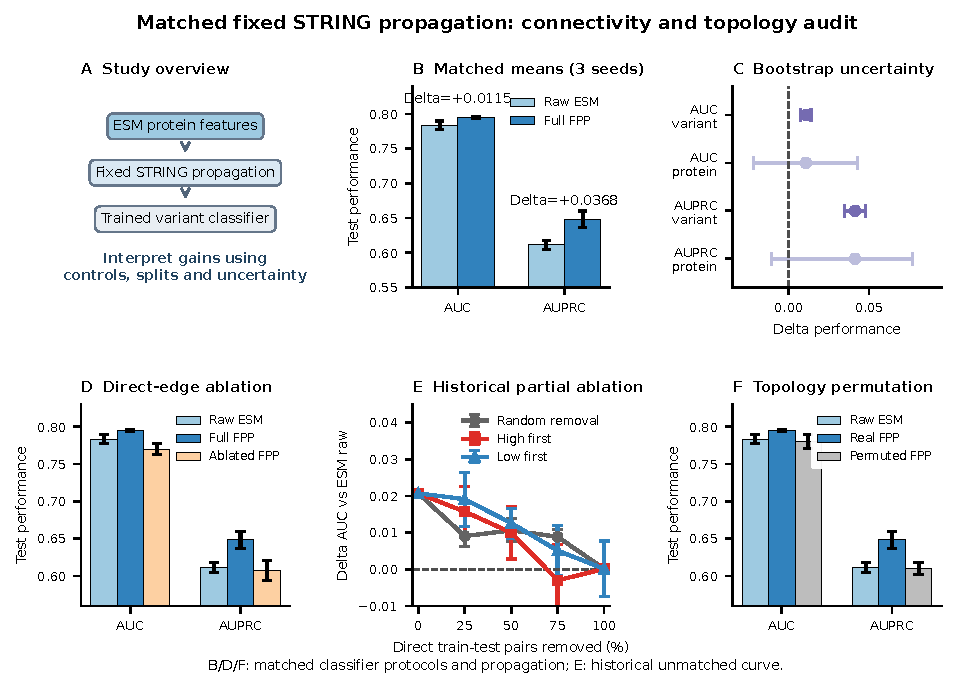
\includegraphics[width=0.98\textwidth]{figure_drafts/Figure1_fixed_propagation_audit.pdf}
\caption{Matched audit of fixed STRING propagation. A, Study overview. B, Raw ESM and full FPP: three classifier seeds per arm, mean and SD. C, Paired bootstrap of ensemble-averaged predictions, comparing variant and protein resampling; 2,000 replicates each. D, Direct-edge ablation with the common propagation operator and matched classifier protocol, mean and SD across three seeds. E, Historical partial-ablation curve with unmatched protocols and reused endpoints; it is not a matched continuation of panel D. F, Three topology permutations by the same three classifier seeds; pooled mean and SD describe both sources of dispersion. New arms share maximum 50 epochs and validation-based early stopping.}
\label{fig:connectivity}
\end{figure*}

\subsection{Architecture-matched fusion and homology-aware stress test}

Under the original split, new architecture-matched \CADDAM{} classifiers reached AUC 0.9572 and AUPRC 0.9072. Adding raw ESM gave 0.9682/0.9326, full FPP 0.9716/0.9409, edge-ablated FPP 0.9704/0.9394 and topology-permuted FPP 0.9692/0.9354 (AUC/AUPRC; Fig. 2B). The protein-clustered interval for the real-minus-raw fusion AUC margin was [+0.0008, +0.0061]. The edge-ablated margin crossed zero, whereas the permutation margin was small and positive conditional on the sampled graphs (Supplementary Table 12); these exploratory comparisons are not multiplicity-adjusted. All arms share hidden layers, preprocessing, seeds, budget and the propagation convention. The score-only arm has fewer input weights despite identical hidden layers. Ensemble-based protein-clustered intervals quantify real-FPP margins over each control (Fig. 2C; Supplementary Table 12); intervals spanning zero establish uncertainty, not equivalence. Pooled permutation dispersion must not be interpreted as nine independent graph replicates.

Under the historical homology-aware representation comparison, FPP gave AUC 0.7606 versus 0.7248 for raw ESM, with AUPRC 0.2768 versus 0.2418 (Fig. 2D). The new symmetric three-seed fusion comparison gave \CADDAM{} AUC 0.9755 $\pm$ 0.0001 and AUPRC 0.8403 $\pm$ 0.0006; adding raw ESM gave 0.9727 $\pm$ 0.0003 and 0.8253 $\pm$ 0.0016; adding FPP gave 0.9752 $\pm$ 0.0007 and 0.8369 $\pm$ 0.0060 (Fig. 2E). The ensemble FPP-minus-score AUC difference was +0.0001, protein-clustered 95\% CI [-0.0019, +0.0021]; the AUPRC difference was -0.0012, CI [-0.0199, +0.0154]. Both intervals span zero, so repeated fitting does not establish a benefit or consistent harm relative to scores alone. Close point rankings can reverse between mean run metrics and metrics of averaged probabilities. This replaces the previous comparison of one graph-fusion run against repeated baselines. Prevalence differs across splits, so AUPRC comparisons remain within-split. Redundant high-dimensional inputs, additional input weights, unscaled features and altered protein composition are possible explanations for fusion behavior; these mechanisms were not distinguished experimentally.

\begin{figure*}[!t]
\centering
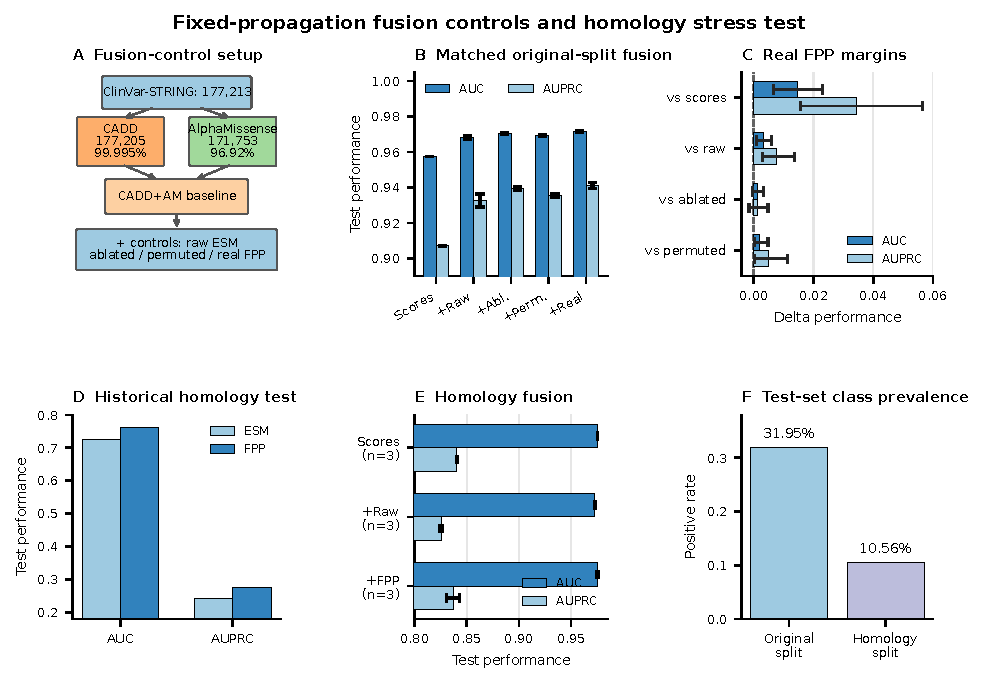
\includegraphics[width=0.98\textwidth]{figure_drafts/Figure2_fusion_homology.pdf}
\caption{Matched fusion and homology-aware evaluation. A, External-score coverage and fusion setup. B, Original-split matched fusion, mean and SD over three seeds per arm; permutation uses three graphs by three seeds. C, Real-FPP minus control performance on ensemble-averaged probabilities, with paired protein-clustered 95\% bootstrap intervals (2,000 replicates). Ensemble point differences can differ from differences of mean run metrics in B. Intervals condition on fitted models and sampled graph permutations; they omit retraining and new-permutation uncertainty. D, Historical retained homology-aware representation estimates. E, New homology-aware fusion: all three arms use the same three seeds, classifier protocol and maximum 50 epochs; error bars indicate SD. F, Test prevalence by split. Scores denotes CADD+AlphaMissense; Raw, Abl., Perm. and Real denote added representations.}
\label{fig:fusion_homology}
\end{figure*}

\subsection{Exploratory topology-context descriptions}

ESM representation space showed weak but detectable correspondence with STRING topology. Sampled STRING-neighbour pairs had mean ESM cosine similarity 0.8789 compared with 0.8639 for random protein pairs, and within-community pairs had higher similarity than between-community pairs (0.8743 versus 0.8642; Fig. 3A). This pattern is consistent with modest correspondence between ESM representation space and STRING network structure before propagation.

Using historical retained-reference predictions, graph-associated gains varied across topology strata without a monotonic centrality pattern. For example, the mid-k-core stratum had $\Delta$ AUC +0.0775, whereas the high-degree stratum had $\Delta$ AUC -0.0178 (Fig. 3B). Betweenness, clustering and neighbour-risk strata also differed descriptively (Fig. 3C,D; Supplementary Table 5). These associations do not establish which biological contexts will benefit on new data.

Joint topology maps provide candidate patterns for later validation (Fig. 3E,F). All 53 joint cells and the highlighted positive and negative profiles were inspected on the same test data. Extreme profiles can therefore arise from sampling variation and subgroup selection. The displayed intervals quantify within-cell resampling only; neither those intervals nor feature-level FDR correction accounts for selection of high-gain cells. The profiles are hypothesis-generating and require independent confirmation.

\begin{figure*}[!t]
\centering
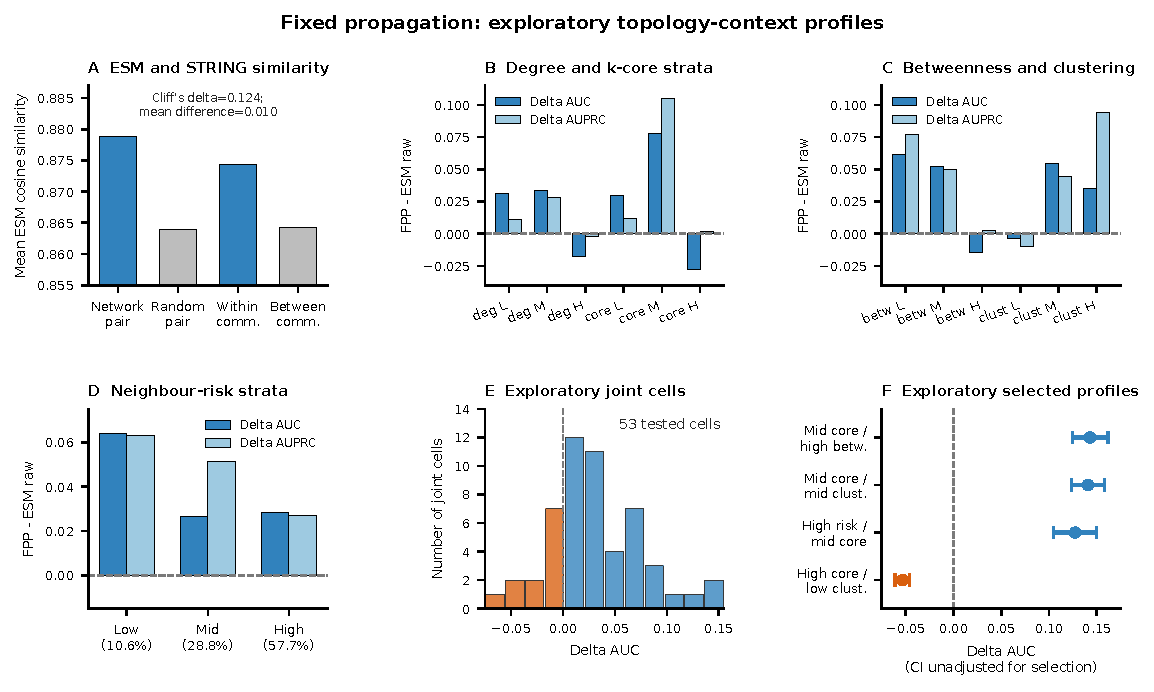
\includegraphics[width=0.98\textwidth]{figure_drafts/Figure3_exploratory_topology.pdf}
\caption{Exploratory descriptions of retained-reference FPP gains across network topology contexts. A, ESM representations show weak alignment with STRING topology. B, Degree and k-core gains are non-monotonic. C, Betweenness and clustering strata shape graph-derived gain. D, Neighbour-risk strata show local-context dependence. E, Exploratory joint-cell distribution. L/M/H denote low/mid/high strata; deg, core, betw and clust denote degree, k-core, betweenness and clustering. F, Exploratory selected profiles; intervals are unadjusted for test-set selection and require independent validation.}
\label{fig:topology_context}
\end{figure*}

\subsection{Graph augmentation reshapes false-negative and false-positive predictions differently}

At a fixed decision-score threshold of 0.5, raw ESM and FPP were jointly correct for 11,875 test variants and jointly wrong for 3,965 variants. FPP corrected 1,436 variants and degraded 944 variants relative to raw ESM. Corrected variants included 837 pathogenic false negatives rescued and 599 benign false positives suppressed, whereas degraded variants included 904 benign true negatives converted to false positives and 40 pathogenic true positives converted to false negatives (Fig. 4A).

The retained-reference \CADDAM{} baseline and graph-fusion model were jointly correct for 15,981 variants and jointly wrong for 1,298 variants; graph fusion corrected 666 variants and degraded 275 variants. The corrected set contained more suppressed false positives than rescued false negatives (444 versus 222; Fig. 4B). Figure 4B uses this retained-reference model pair, while Figure 2 reports the architecture-matched repeated-run comparison.

In this exploratory comparison, topology profiles differed between rescued false negatives and suppressed false positives. In the raw ESM to FPP comparison, rescued false negatives had higher degree, neighbour-risk, neighbour pathogenic rate, neighbour training-variant count and betweenness; suppressed false positives had higher clustering coefficient and within-community neighbour fraction (Fig. 4C). Similar profile shifts appeared in the retained \CADDAM{} to graph-fusion comparison (Fig. 4D). Multiple topology features remained significant after FDR correction (Fig. 4E), and baseline-error-stratified contrasts showed differences across degree, k-core, neighbour-risk, neighbour pathogenic rate, betweenness and boundary role (Fig. 4F). These are descriptive associations within baseline false-negative or false-positive groups, without continuous-score matching. A post-hoc threshold sweep from 0.1 to 0.9 (Supplementary Table 10) found net corrections of -234 at 0.1 and +10 to +587 at 0.2--0.9 for raw ESM to FPP. The retained fusion pair had positive net corrections throughout, but its dominant corrected error type reversed at 0.7. Thus the detailed error-type story at 0.5 is threshold-dependent.

\begin{figure*}[!t]
\centering
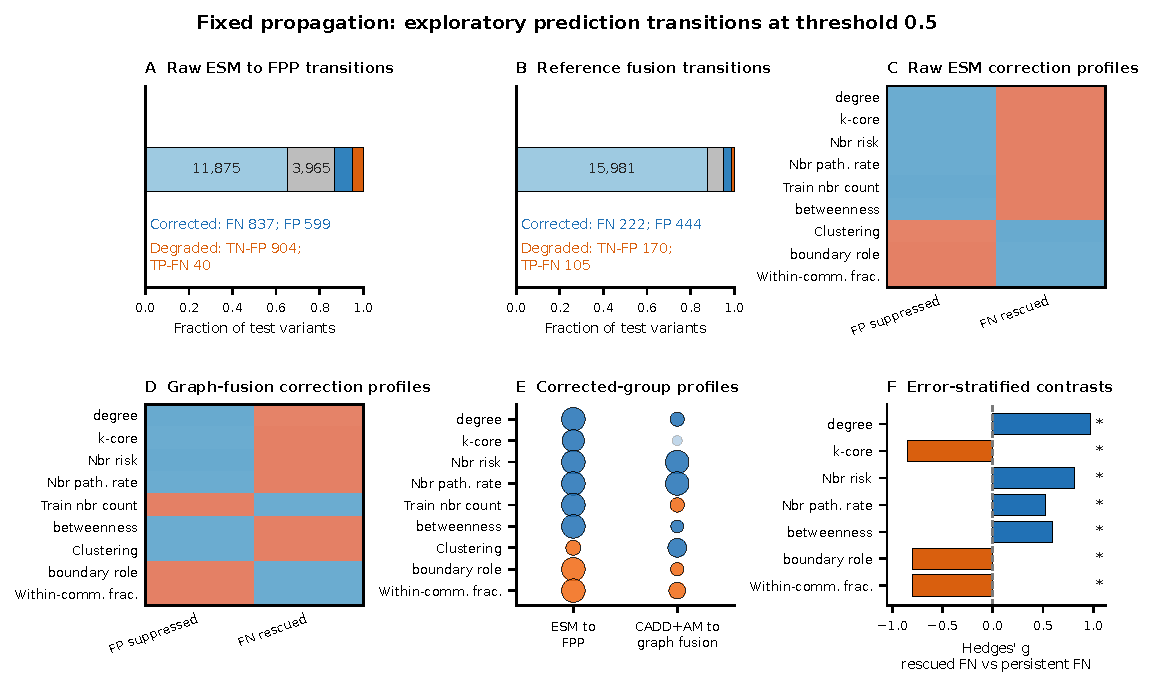
\includegraphics[width=0.98\textwidth]{figure_drafts/Figure4_prediction_transitions.pdf}
\caption{Graph augmentation changes false-negative and false-positive predictions in different network contexts. A, Transitions for the historical retained raw-ESM/FPP pair at score threshold 0.5. B, Transitions for the retained-reference \CADDAM{} and graph-fusion model pair. C-D, Row-normalized heatmaps compare topology profiles of suppressed false positives and rescued false negatives. E, Corrected groups differ across multiple topology features after FDR correction. F, Baseline-error-stratified contrasts, without continuous-score matching. Nbr denotes neighbour; path. rate is training-neighbour pathogenic rate. Counts are threshold-specific and sigmoid outputs are uncalibrated; see Supplementary Table 10.}
\label{fig:prediction_transitions}
\end{figure*}

\section{Discussion}

This audit concerns fixed feature propagation on one STRING association network. The original-split mean performance improved over raw ESM, with protein-clustered intervals spanning zero, and the new connectivity and identity-permutation controls use matched training protocols and propagation operators. These controls test sensitivity to graph interventions; they do not identify a purely causal connectivity effect. Shared graph structure and held-out protein features are permitted by the transductive design. No test labels enter propagation, but deployment to newly arriving, disconnected proteins is not evaluated.

Architecture-matched fusion compares adding representations with adding classifier capacity. The new matched results update the original fusion comparisons; historical complete-case test-subset checks remain in Supplementary Table 9, with current fitted-prediction sensitivity in Table 13. Neither is a complete-case training experiment. They do not provide an independent validation cohort. Small network-specific margins require protein-level uncertainty rather than only point ordering.

The external predictors are not independent prospective references. CADD uses proxy-neutral versus simulated proxy-deleterious training examples and incorporates ESM-1v features \cite{Kircher2014CADD,Schubach2024CADDv17}; AlphaMissense uses population-derived weak supervision and clinical variants for model selection and calibration \cite{Cheng2023AlphaMissense}. Clinical-data involvement in development differs from direct supervised training on our labels. Historical clinical overlap was not enumerated or excluded here. A temporal cohort excluding predictor-development variants is needed before interpreting these comparisons as prospective generalization.

The homology-aware split changes protein composition and prevalence. Its new matched three-seed fusion comparison resolves the previous unequal repeat count, but one frozen partition and three seeds do not establish generality across homology partitions or prospective cohorts. Prevalence-controlled comparisons remain outside this study. The topology profiles and error transitions are exploratory; independent data must test subgroup reproducibility, and threshold-dependent transitions must not be treated as calibrated clinical improvements.

Several further boundaries matter. STRING combines functional associations beyond physical interactions; physical-only and alternative networks were not tested \cite{Szklarczyk2023STRING}. Fixed propagation may be inadequate to extract useful topology even when that topology is informative. The supplementary mean and cosine-weighted operators are also fixed: they are not trained GraphSAGE or GAT baselines. Learned attention, heterogeneous variant graphs and context-aware models therefore remain outside the scope of the present conclusions. Protein-level features omit mutation identity and isoform effects, while ClinVar submission bias, changing labels and the review-status whitelist limit transfer \cite{Landrum2020ClinVar}. Binary labels discard graded functional effects; stricter/looser training filters and independent functional assays were not evaluated. Computational pathogenicity predictions require clinical or functional confirmation and cannot alone establish diagnosis or treatment.

\paragraph{Practical recommendations}
Evaluate fixed propagation against raw protein features and capacity-matched score baselines on the intended split. Match classifier seeds and training budgets, report cross-partition graph access, and quantify uncertainty at the protein level. Treat unmatched controls as descriptive and validate selected subgroups independently. Assess thresholds and calibration before interpreting prediction changes as useful decision rules.

\section{Conclusion}
Fixed STRING propagation shows evaluation-dependent gains on this ClinVar cohort. Graph controls and strong baselines are essential to interpret those gains. The present evidence neither establishes a performance ceiling nor determines how trained graph models or independent cohorts would behave.

\section*{Data and Code Availability}

The public repository \url{https://github.com/brynn-t02/ppi-graph-missense-audit} contains the historical scripts and the 8 and 23 October revision snapshots. This revision additionally supplies its matched-experiment code, runtime records, per-run metrics, predictions and input checksums as a local reproducibility package; upload of these new additions has not yet been verified. Large-scale reconstruction and training require the original provider resources and an appropriate compute environment. ClinVar, STRING, CADD and AlphaMissense resources should be obtained from their providers.

\section*{AI-Tool Disclosure}

OpenAI ChatGPT, OpenAI Codex and Anthropic Claude supported literature organization, analysis-code drafting and language editing. Historical experiments were performed by the authors. Revision-stage scripts assisted by these tools restored an isolated runtime, checked input provenance, trained matched downstream classifiers on the provided data, and recomputed sensitivity statistics. Actual logs, fitted predictions and checksums are retained for review. The authors retain responsibility for study design, interpretation, citation verification and final approval. The tools are not authors; no synthetic outcomes were substituted for experimental results.

\begin{thebibliography}{99}
\bibitem{Barabasi2011NetworkMedicine} A.-L. Barabasi, N. Gulbahce, and J. Loscalzo, ``Network medicine: a network-based approach to human disease,'' \emph{Nature Reviews Genetics}, vol. 12, pp. 56--68, 2011, doi: 10.1038/nrg2918.
\bibitem{Benjamini1995FDR} Y. Benjamini and Y. Hochberg, ``Controlling the false discovery rate: a practical and powerful approach to multiple testing,'' \emph{Journal of the Royal Statistical Society: Series B}, vol. 57, pp. 289--300, 1995, doi: 10.1111/j.2517-6161.1995.tb02031.x.
\bibitem{Chen2018InteractomePerturbation} S. Chen et al., ``An interactome perturbation framework prioritizes damaging missense mutations for developmental disorders,'' \emph{Nature Genetics}, vol. 50, pp. 1032--1040, 2018, doi: 10.1038/s41588-018-0130-z.
\bibitem{Cheng2021VEGN} J. Cheng, C. Lawrence, and M. Niepert, ``VEGN: variant effect prediction with graph neural networks,'' arXiv:2106.13642, 2021, doi: 10.48550/arXiv.2106.13642.
\bibitem{Cheng2023AlphaMissense} J. Cheng et al., ``Accurate proteome-wide missense variant effect prediction with AlphaMissense,'' \emph{Science}, vol. 381, eadg7492, 2023, doi: 10.1126/science.adg7492.
\bibitem{Efron1993Bootstrap} B. Efron and R. J. Tibshirani, \emph{An Introduction to the Bootstrap}. Chapman \& Hall/CRC, 1993.
\bibitem{Frazer2021EVE} J. Frazer et al., ``Disease variant prediction with deep generative models of evolutionary data,'' \emph{Nature}, vol. 599, pp. 91--95, 2021, doi: 10.1038/s41586-021-04043-8.
\bibitem{Ghadie2025DiseaseSpecificGNN} M. Ghadie, S. Sardaar, and Y. Trakadis, ``Disease-specific prediction of missense variant pathogenicity with DNA language models and graph neural networks,'' \emph{Bioengineering}, vol. 12, p. 1098, 2025, doi: 10.3390/bioengineering12101098.
\bibitem{Ioannidis2016REVEL} N. M. Ioannidis et al., ``REVEL: an ensemble method for predicting the pathogenicity of rare missense variants,'' \emph{American Journal of Human Genetics}, vol. 99, pp. 877--885, 2016, doi: 10.1016/j.ajhg.2016.08.016.
\bibitem{Kingma2015Adam} D. P. Kingma and J. Ba, ``Adam: a method for stochastic optimization,'' \emph{International Conference on Learning Representations}, 2015, arXiv:1412.6980.
\bibitem{Kipf2017GCN} T. N. Kipf and M. Welling, ``Semi-supervised classification with graph convolutional networks,'' \emph{International Conference on Learning Representations}, 2017.
\bibitem{Kircher2014CADD} M. Kircher et al., ``A general framework for estimating the relative pathogenicity of human genetic variants,'' \emph{Nature Genetics}, vol. 46, pp. 310--315, 2014, doi: 10.1038/ng.2892.
\bibitem{Landrum2020ClinVar} M. J. Landrum et al., ``ClinVar: improvements to accessing data,'' \emph{Nucleic Acids Research}, vol. 48, pp. D835--D844, 2020, doi: 10.1093/nar/gkz972.
\bibitem{Lin2023ESM} Z. Lin et al., ``Evolutionary-scale prediction of atomic-level protein structure with a language model,'' \emph{Science}, vol. 379, pp. 1123--1130, 2023, doi: 10.1126/science.ade2574.
\bibitem{Littmann2022ProteinMLTips} Q. Hou, K. Waury, D. Gogishvili, and K. A. Feenstra, ``Ten quick tips for sequence-based prediction of protein properties using machine learning,'' \emph{PLOS Computational Biology}, vol. 18, no. 12, Art. no. e1010669, 2022, doi: 10.1371/journal.pcbi.1010669.
\bibitem{Menche2015DiseaseModules} J. Menche et al., ``Disease networks. Uncovering disease-disease relationships through the incomplete interactome,'' \emph{Science}, vol. 347, 1257601, 2015, doi: 10.1126/science.1257601.
\bibitem{Ozturk2022NetworkFeatures} K. Ozturk and H. Carter, ``Predicting functional consequences of mutations using molecular interaction network features,'' \emph{Human Genetics}, vol. 141, pp. 1195--1210, 2022, doi: 10.1007/s00439-021-02329-5.
\bibitem{Qi2021MVP} H. Qi et al., ``MVP predicts the pathogenicity of missense variants by deep learning,'' \emph{Nature Communications}, vol. 12, p. 510, 2021, doi: 10.1038/s41467-020-20847-0.
\bibitem{Sahni2015InteractionPerturbation} N. Sahni et al., ``Widespread macromolecular interaction perturbations in human genetic disorders,'' \emph{Cell}, vol. 161, pp. 647--660, 2015, doi: 10.1016/j.cell.2015.04.013.
\bibitem{Saito2015PrecisionRecall} T. Saito and M. Rehmsmeier, ``The precision-recall plot is more informative than the ROC plot when evaluating binary classifiers on imbalanced datasets,'' \emph{PLOS ONE}, vol. 10, e0118432, 2015, doi: 10.1371/journal.pone.0118432.
\bibitem{Schubach2024CADDv17} M. Schubach et al., ``CADD v1.7: using protein language models, regulatory CNNs and other nucleotide-level scores to improve genome-wide variant predictions,'' \emph{Nucleic Acids Research}, vol. 52, no. D1, pp. D1143--D1154, 2024, doi: 10.1093/nar/gkad989.
\bibitem{Steinegger2017MMseqs2} M. Steinegger and J. Soding, ``MMseqs2 enables sensitive protein sequence searching for the analysis of massive data sets,'' \emph{Nature Biotechnology}, vol. 35, pp. 1026--1028, 2017, doi: 10.1038/nbt.3988.
\bibitem{Sundaram2018PrimateAI} L. Sundaram et al., ``Predicting the clinical impact of human mutation with deep neural networks,'' \emph{Nature Genetics}, vol. 50, pp. 1161--1170, 2018, doi: 10.1038/s41588-018-0167-z.
\bibitem{Szklarczyk2023STRING} D. Szklarczyk et al., ``The STRING database in 2023: protein-protein association networks and functional enrichment analyses for any sequenced genome of interest,'' \emph{Nucleic Acids Research}, vol. 51, pp. D638--D646, 2023, doi: 10.1093/nar/gkac1000.
\bibitem{Teufel2023GraphPart} F. Teufel, M. H. Gislason, J. J. Almagro Armenteros, A. R. Johansen, O. Winther, and H. Nielsen, ``GraphPart: homology partitioning for biological sequence analysis,'' \emph{NAR Genomics and Bioinformatics}, vol. 5, lqad088, 2023, doi: 10.1093/nargab/lqad088.
\bibitem{Yates2014SuSPect} C. M. Yates, I. Filippis, L. A. Kelley, and M. J. E. Sternberg, ``SuSPect: enhanced prediction of single amino acid variant phenotype using network features,'' \emph{Journal of Molecular Biology}, vol. 426, pp. 2692--2701, 2014, doi: 10.1016/j.jmb.2014.04.026.
\bibitem{Yu2025GNNMAP} H. Yu et al., ``A graph neural network approach for accurate prediction of pathogenicity in multi-type variants,'' \emph{Briefings in Bioinformatics}, vol. 26, bbaf151, 2025, doi: 10.1093/bib/bbaf151.
\bibitem{Zhang2022gMVP} H. Zhang, M. S. Xu, X. Fan, W. K. Chung, and Y. Shen, ``Predicting functional effect of missense variants using graph attention neural networks,'' \emph{Nature Machine Intelligence}, vol. 4, no. 11, pp. 1017--1028, 2022, doi: 10.1038/s42256-022-00561-w.
\end{thebibliography}
\end{document}
